\subsection{Measurements}

A dual-stacked user when attempting to connect to a dual-stacked service
traditionally prefers connecting over IPv6. This is because in POSIX systems,
the internal domain name resolution system call \texttt{getaddrinfo(\ldots)}
\cite{rfc3493} returns the list of addresses in an order that prioritizes an
IPv6-upgrade path \cite{rfc6724}. The dictated order can dramatically reduce
the application responsiveness in situations where IPv6 connectivity is
broken. This is because, the attempt to connect over an IPv4 address will take
place only when the IPv6 connection attempt has timed out, which can be in the
order of seconds.

This noticeable degraded user experience can be subverted by making
applications apply the happy eyeballs algorithm \cite{rfc6555}. The algorithm
recommends that a dual-stacked application try resolving a dual-stacked
service for both IPv4 and IPv6 addresses at once. If the resolver returns both
addresses, the application must try a TCP \texttt{connect(\ldots)} to both the
resolved addresses and pick the one that completes first.

In this pursuit, to determine whether applications will use IPv4 or IPv6 on a
dual stacked service, we developed \texttt{happy}, a simple TCP happy eyeballs
probing tool. It uses non-blocking \texttt{connect(\ldots)} calls to establish
concurrent connections to a number of possible endpoints of a service. The
tool, however, does not check whether the endpoints of a given target all
provide the same service. Hence, it is possible to impact the results by
setting up fake servers that do not provide the service tested and which are
designed and deployed with the only purpose to provide fast connection setup
times.

We have cross-compiled \texttt{happy} for the OpenWRT \cite{fainelli:2008}
platform. As a result, the tool can now be run on widely deployed SamKnows
probes \footnote{\url{http://www.samknows.com}}, and the collected measurement
data can be further analysed. In order to ascertain the value in this
exercise, we prepared an internal test-bed of multiple measurement points. The
measurement points have different flavors of IPv4 and IPv6 connectivity
ranging from native IPv4, native IPv6, IPv6 tunnel broker endpoints
\cite{rfc3053}, Teredo \cite{rfc4380} and tunnelled IPv4. We used the top 100
domains compiled by Hurricane Electric Internet Services
\footnote{\url{http://bgp.he.net/ipv6-progress-report.cgi}} and ran
\texttt{happy} on the set of dual-stack services represented by these domains.
A preliminary result comparing the time (mean and standard deviation) to make
a TCP connection to each of these services over IPv4 and IPv6 is shown in Fig.
\ref{fig:happy-servers-mean-std}. The measurement point represented in this
plot is located at Braunschweig and has a native IPv4 and a IPv6 connection
through the German Research Network \footnote{\url{http://www.dfn.de}}. The
initial results show higher time variances when connections are made over
IPv6. In addition, some of the related (and few of the unrelated) services
show similar mean and standard deviations. These services either resolve to
the same endpoint or a set of endpoints that belong to an allocated block.
Digging through the \texttt{whois} information for each of the endpoints from
their \ac{RIR} seems to indicate that major portion of the services map to a
cloud of an address block owned by popular organizations like Google and
Akamai Technologies as shown in Fig. \ref{fig:v4-v6-cloud}.

\begin{figure}[t]
\centering
\includegraphics*[width=1.0\linewidth]{figures/happy-servers-mean-std}
\caption{servers vs \texttt{\{mean, std\}}}
\label{fig:happy-servers-mean-std}
\end{figure}

\begin{figure}
  \begin{minipage}[h]{0.50\textwidth}
    \centering
    \resizebox*{1.0\textwidth}{!}{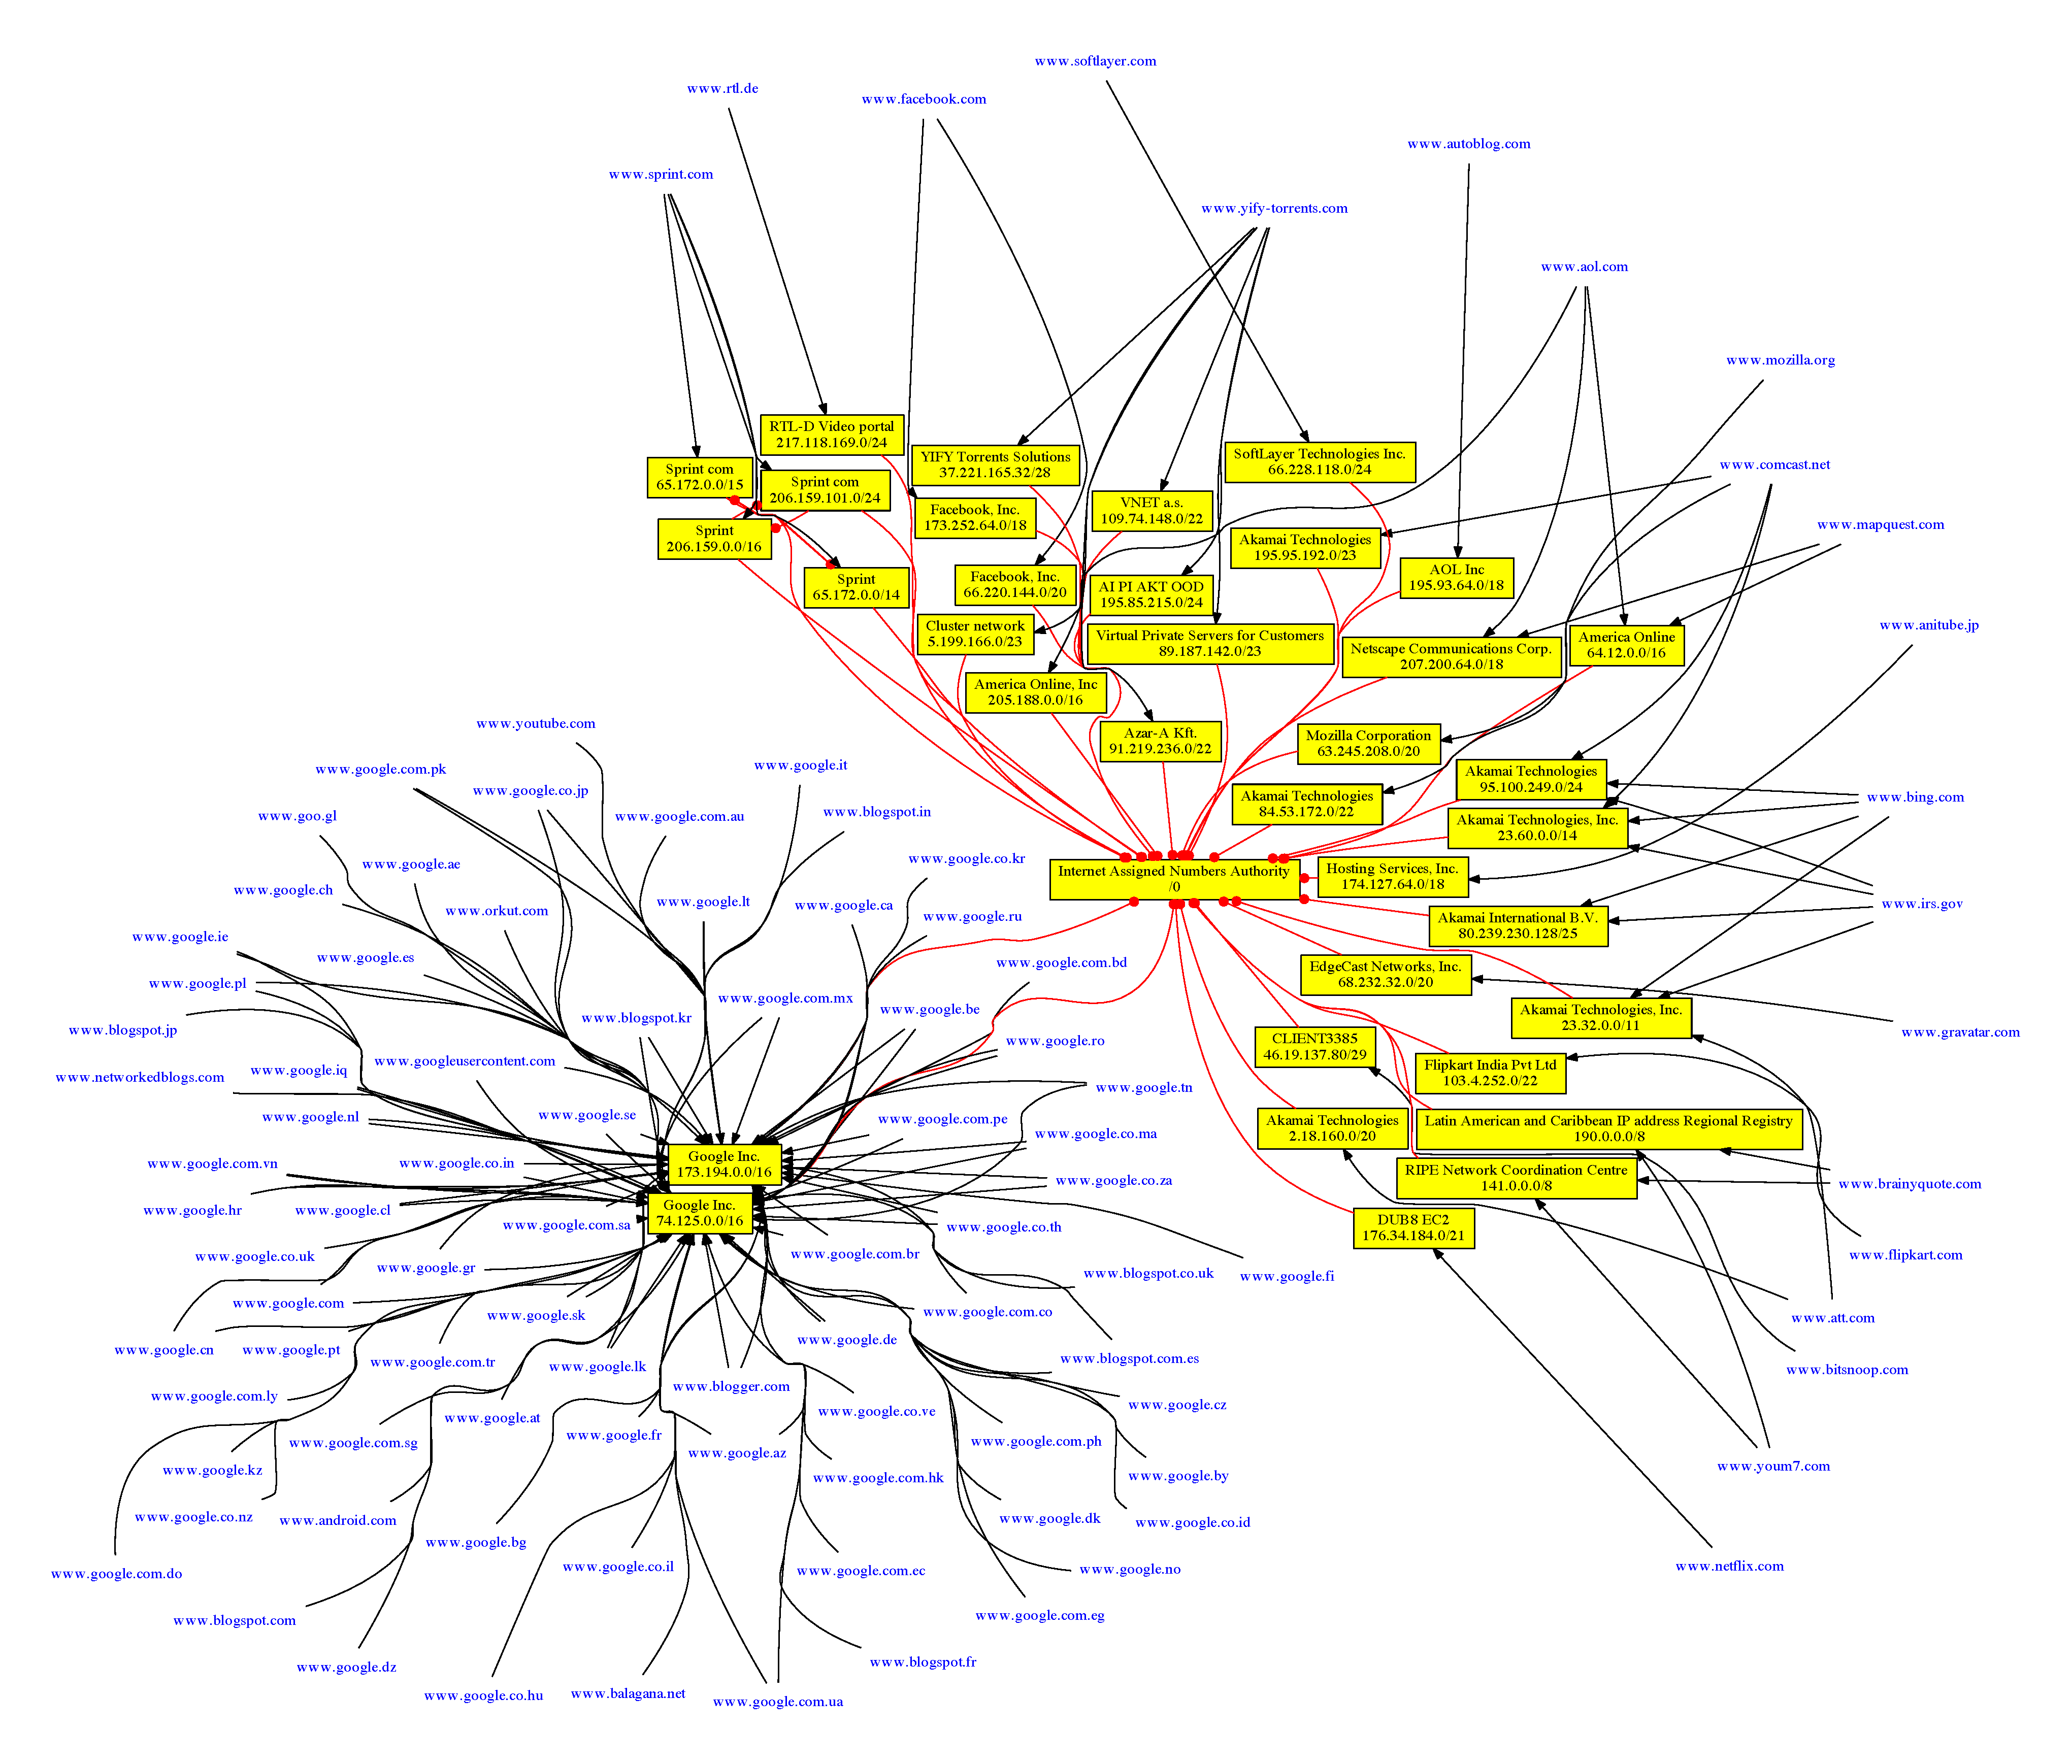
\includegraphics{figures/happy-v4cloud}}
  \end{minipage}
  \begin{minipage}[h]{0.50\textwidth}
    \centering
    \resizebox*{1.0\textwidth}{!}{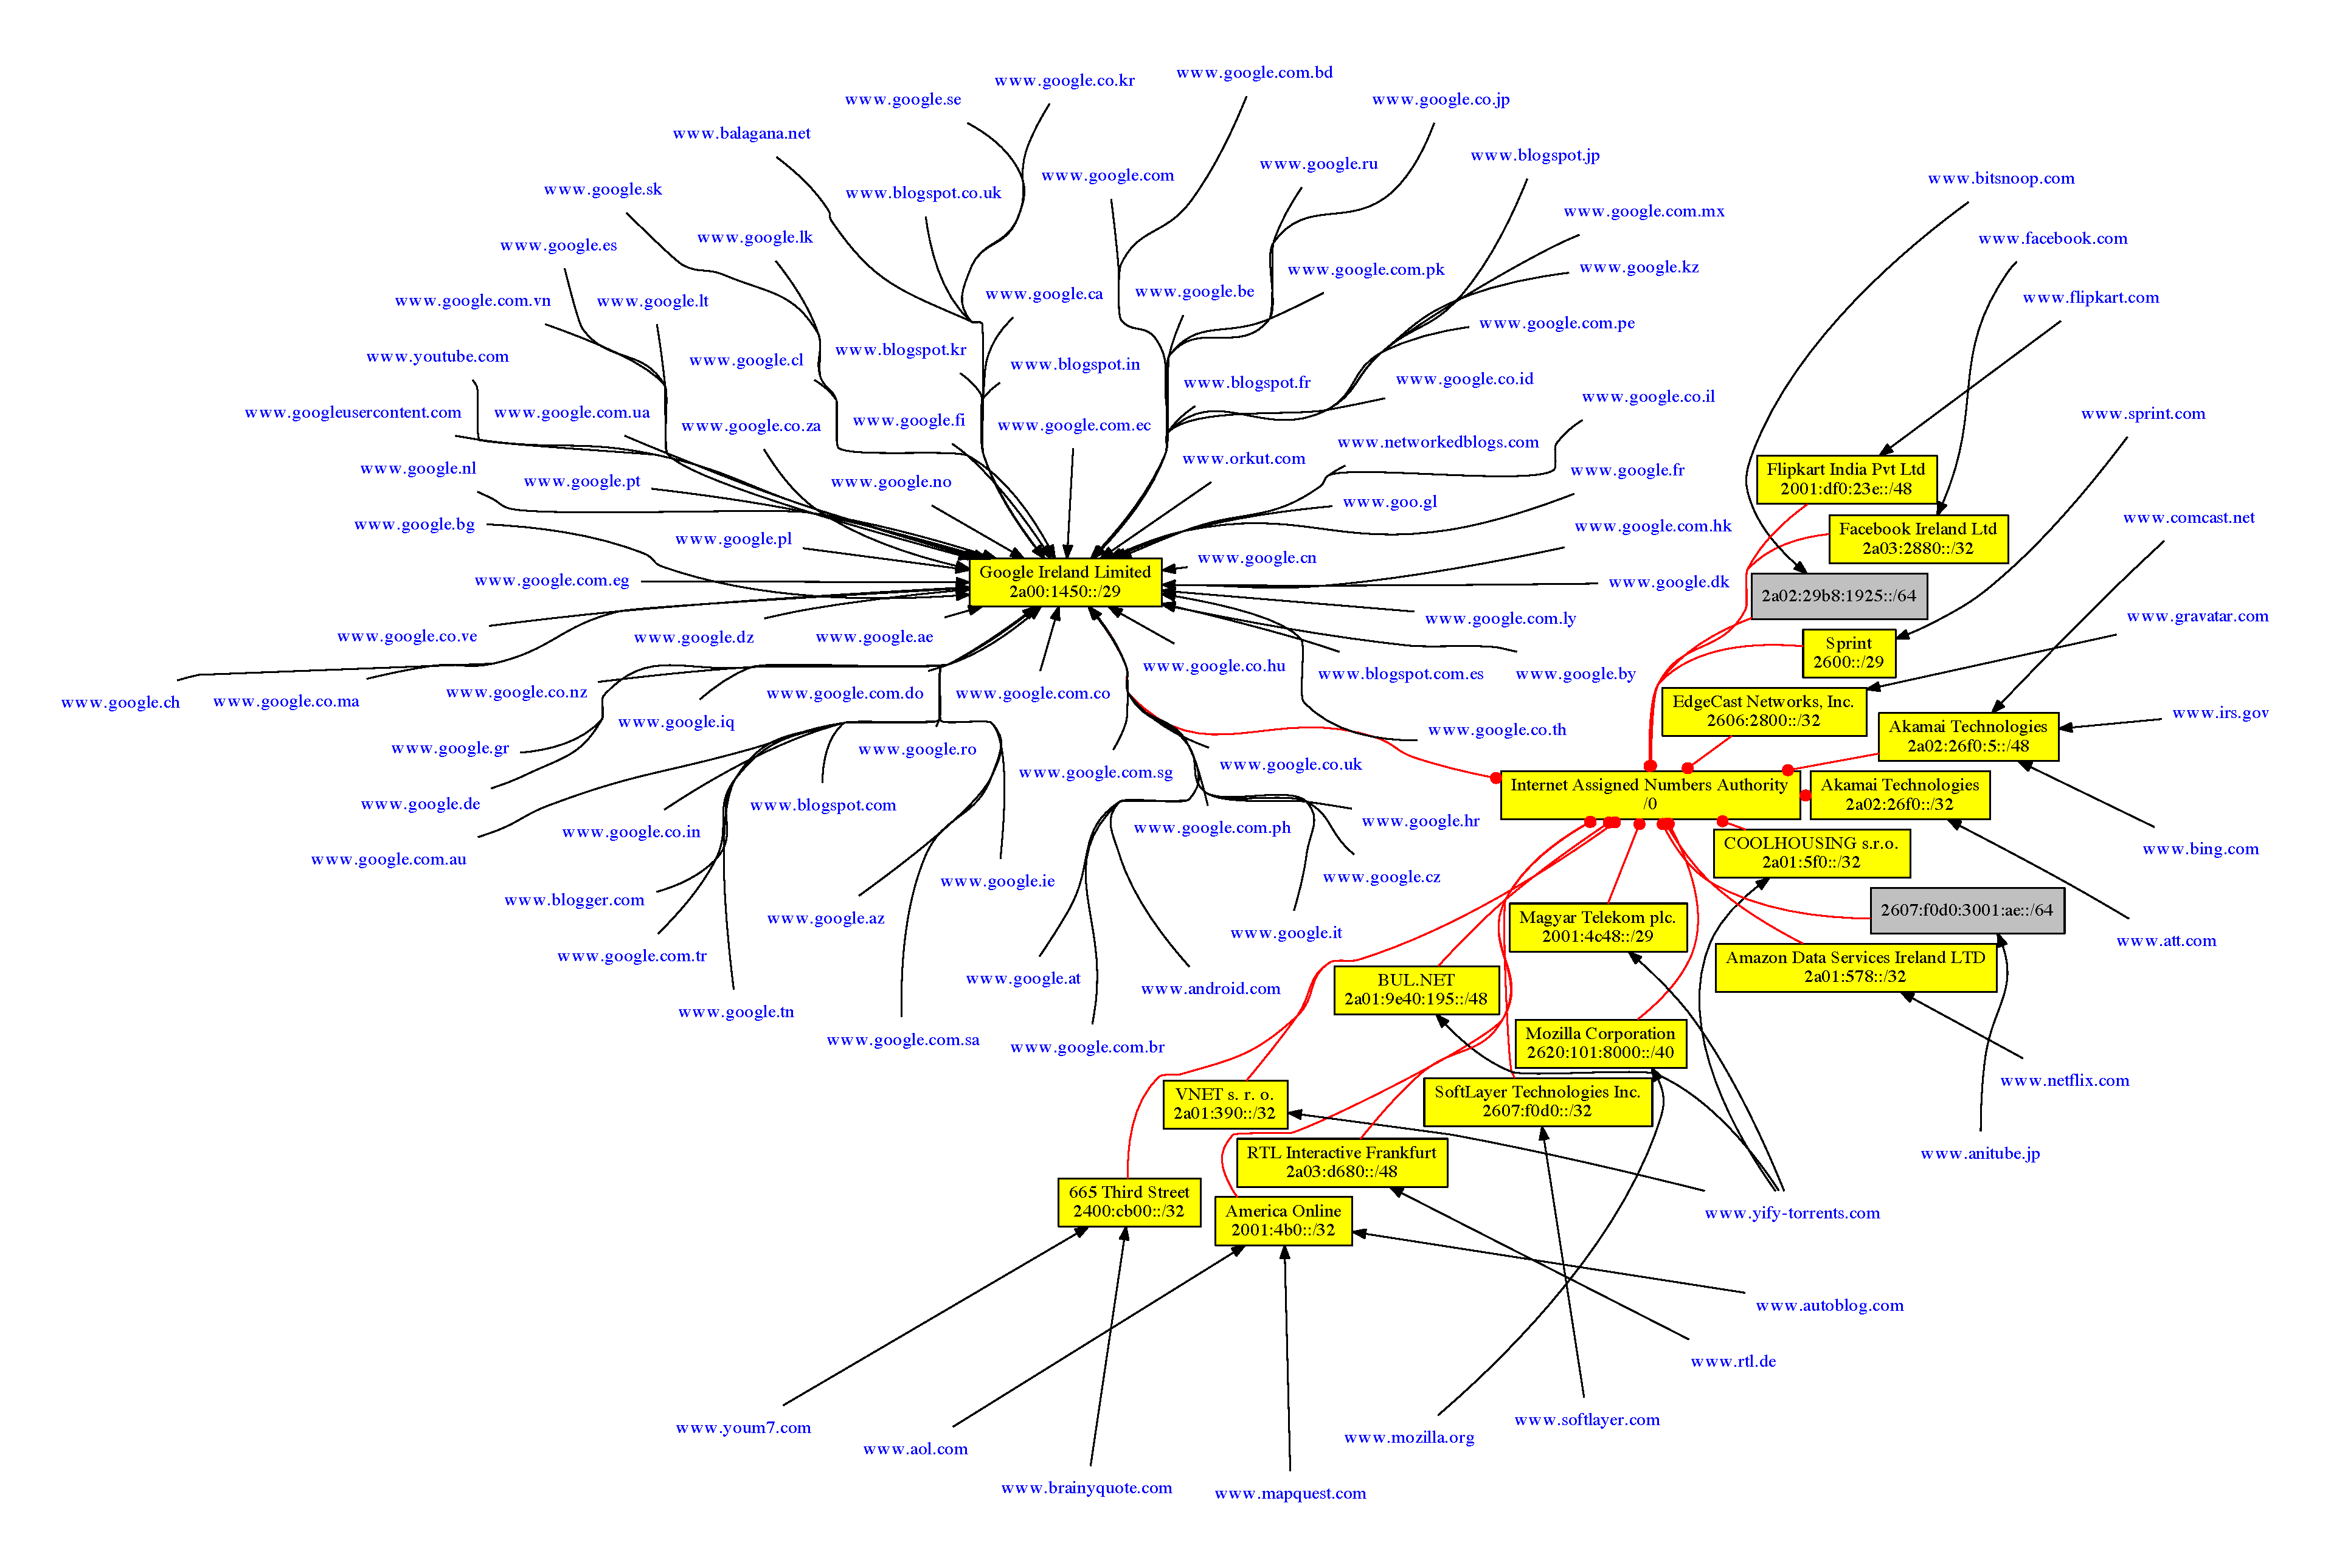
\includegraphics{figures/happy-v6cloud}}
  \end{minipage}
\caption{\label{fig:v4-v6-cloud}IPv4 and IPv6 aggregation cloud}
\end{figure}

\subsection{Local Management}
